
%(BEGIN_QUESTION)
% Copyright 2011, Tony R. Kuphaldt, released under the Creative Commons Attribution License (v 1.0)
% This means you may do almost anything with this work of mine, so long as you give me proper credit

Suppose a FOUNDATION Fieldbus level transmitter will be used to measure the volume of water stored in a process vessel above the datum line.  The transmitter is connected to the vessel through an impulse tube connected to the ``High'' port of the DP sensor, sensing liquid level directly in units of {\it inches water column}.  The operator, in turn, expects to be able to read liquid volume in {\it gallons}.  The vessel is cylindrical in shape, with a diameter of 40 inches:

$$\includegraphics[width=15.5cm]{i00354x01.eps}$$

Complete the configuration table in the above illustration, showing the proper {\tt XD\_Scale}, {\tt OUT\_Scale}, and {\tt L\_Type} parameter values to make the transmitter function as it should in this application.

\vskip 10pt

Also, determine the proper settings (open or shut) for the three hand valves between the process vessel and the transmitter while the system is operating normally.


\vskip 20pt \vbox{\hrule \hbox{\strut \vrule{} {\bf Suggestions for Socratic discussion} \vrule} \hrule}

\begin{itemize}
\item{} Describe the purpose of the {\tt XD\_Scale} and {\tt OUT\_Scale} parameters in a Fieldbus instrument.
\item{} Explain what will happen if the {\tt L\_Type} parameter is set to {\it Direct}.
\end{itemize}

\underbar{file i00354}
%(END_QUESTION)





%(BEGIN_ANSWER)

Probably the trickiest portion of this problem is how to calculate the volume in gallons, based on nothing but the {\it height} of water as measured by the level transmitter.  Suffice to say, this is fundamentally a geometry problem, followed by a units-conversion problem!

%(END_ANSWER)





%(BEGIN_NOTES)

With a diameter of 40 inches, this vessel has a cross-sectional area equal to:

$$A = \pi r^2$$

$$A = \pi (20 \hbox{ in})^2$$

$$A = 1256.6 \hbox{ in}^2$$

With a vertical water column 55 inches high at this cross-sectional area, the volume of liquid stored at the URV will be:

$$V = A h$$

$$V = \left(1256.6 \hbox{ in}^2\right) (55 \hbox{ in})$$

$$V = 69115.0 \hbox{ in}^3$$

Converting this volume into units of gallons:

$$\left(69115.0 \hbox{ in}^3 \over 1 \right) \left(1 \hbox{ gal} \over 231 \hbox{ in}^3 \right) = 299.2 \hbox{ gal}$$

\vskip 10pt

Knowing that a raw measurement range of 0 to 55 inches water column is equivalent to a volume range of 0 to 299.2 gallons, we may configure the Fieldbus transmitter as follows:

\vskip 10pt

{\tt XD\_Scale} = 0 to 55 inches

\vskip 10pt

{\tt OUT\_Scale} = 0 to 299.2 gallons

\vskip 10pt

{\tt L\_Type} = Indirect

\vskip 10pt

The two block valves should be open and the bleed valve shut during normal operation.


%INDEX% Fieldbus, instrument ranging: setting XD_Scale and OUT_Scale parameters for an application

%(END_NOTES)


